% ------------------------------------------------------------------------
% ------------------------------------------------------------------------
% ------------------------------------------------------------------------
%                                Capítulo 4
% ------------------------------------------------------------------------
% ------------------------------------------------------------------------
% ------------------------------------------------------------------------

\chapter{SIMULACIONES Y RESULTADOS}

En esta sección, se presentan los resultados obtenidos a partir del método propuesto para la clasificación de objetos basado en medidas medidas cuadráticas codificadas comparado con esquemas de clasificación del estado del arte.

\section{CONJUNTO DE DATOS}

Durante el desarrollo de este trabajo, no se encontraron conjuntos de datos públicos enfocados en la clasificación de medidas cuadráticas. Debido a esto, se decidió simular la propagación de las medidas usando conjuntos de datos tradicionales. Para esto se usaron imágenes de los conjuntos de datos MNIST \myfootcite{deng2012mnist} y Fashion-MNIST \myfootcite{xiao2017fashion}. La Figura \ref{fig:conjunto_datos} muestra un ejemplo de diferentes La Tabla \ref{tab:conjunto_datos} muestra la división de datos en entrenamiento, validación y prueba. Cada imagen fue escalada en el rango de $[-\pi, \pi]$ y usada como información de fase de la forma $\mathbf{x}=e^{j\mathrm{ang}(\mathbf{x})}$, donde $j$ representa la unidad imaginaria en el plano complejo.

\begin{figure}[!h]
    \centering
    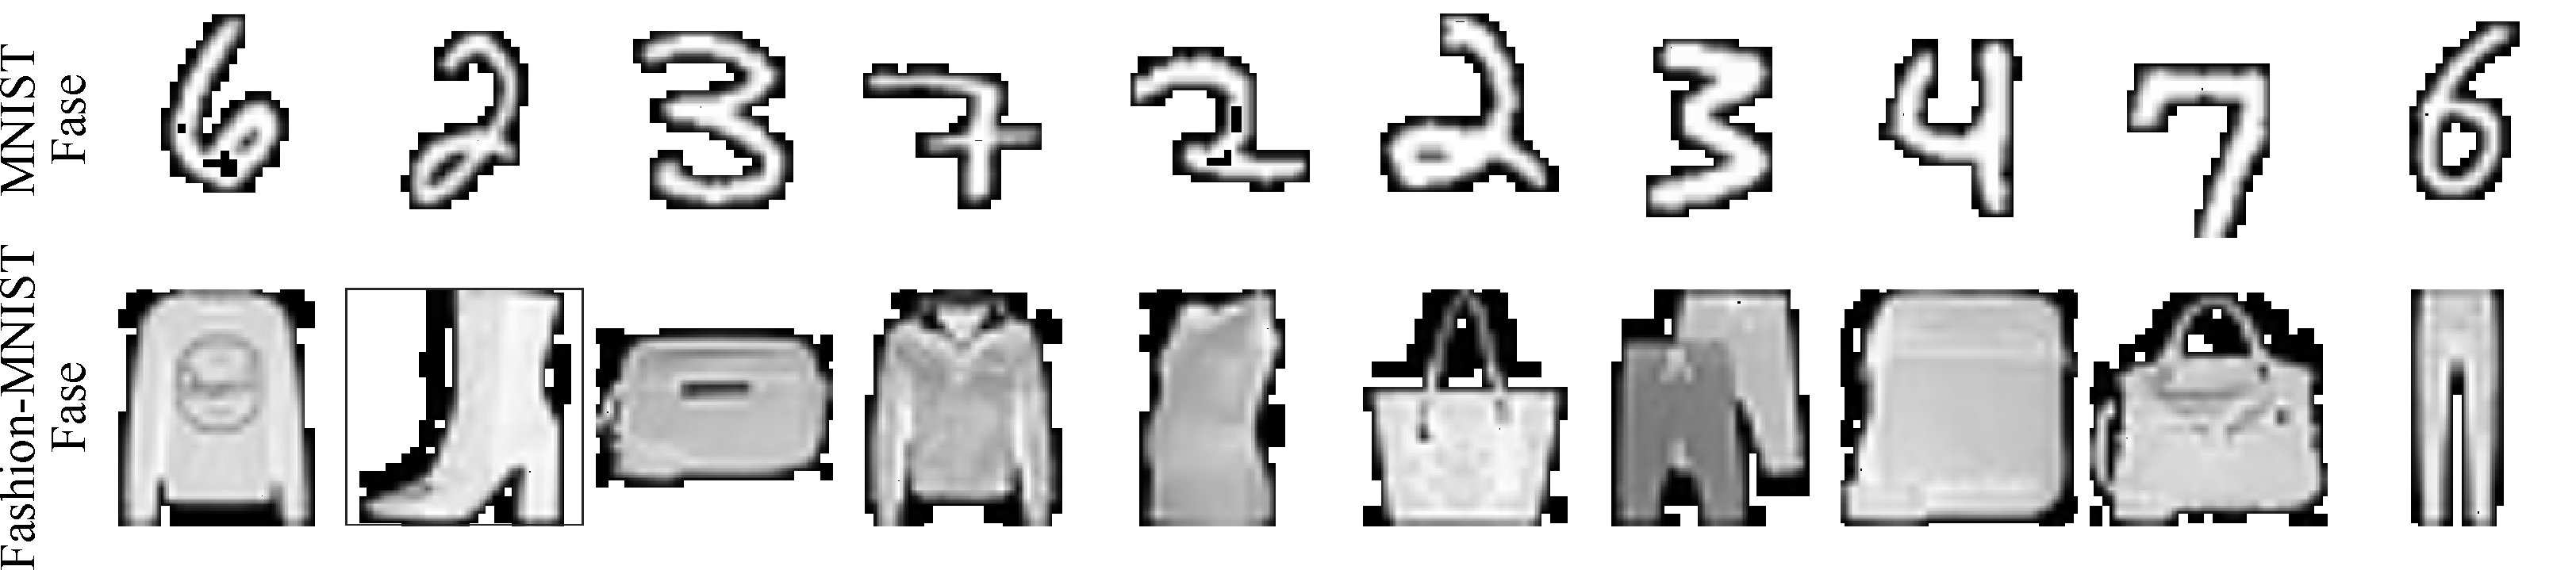
\includegraphics[width=\linewidth]{images/resultados/datasets.pdf}
    \caption{Ejemplo de las imágenes presentes en los conjuntos de datos MNIST y Fashion-MNIST.}
    \label{fig:conjunto_datos}
\end{figure}


% Please add the following required packages to your document preamble:
% \usepackage{graphicx}
\begin{table}[!h]
\centering\scalebox{0.9}{
\resizebox{\textwidth}{!}{%
\begin{tabular}{|c|c|c|c|c|}
\hline
\textbf{Conjunto de datos} & \textbf{Entrenamiento} & \textbf{Validación} & \textbf{Prueba} & \textbf{Total} \\ \hline
MNIST                      & 54000                  & 6000                & 10000           & 70000          \\ \hline
Fashion-MNIST              & 54000                  & 6000                & 10000           & 70000          \\ \hline
\end{tabular}%
}}\caption{Resumen de la división de los conjuntos de datos usados para evaluar el método propuesto.}
\label{tab:conjunto_datos}
\end{table}

\section{MÉTRICAS}
La calidad de la inicialización y la precisión de la clasificación en sistemas de difracción basados en medidas cuadráticas codificadas se mide a través de las siguientes métricas.
\subsection{Métricas para evaluar la inicialización}

Aquí, se describen las métricas usadas para evaluar la estimación inicial $\hat{\mathbf{z}}$ respecto a la imagen de referencia $\mathbf{z}$.
\begin{itemize}
    \item Medida del índice de similitud estructural (SSIM):
    
    \begin{equation}
        %\nonumber
        \mathrm{SSIM}(\mathbf{z}, \tilde{\mathbf{z}}) = \frac{2(\mu_{\mathbf{z}}\mu_{\tilde{\mathbf{z}}} + C_1) + (2\sigma_{\mathbf{z}\tilde{\mathbf{z}}} + C_2)}{(\mu_{\mathbf{z}} + \mu_{\tilde{\mathbf{z}}} + C_1)(\sigma_{\mathbf{z}}\sigma_{\tilde{\mathbf{z}}} + C_1)},
        \label{eq:SSIM}
    \end{equation}
    
    donde $(\mu_{\mathbf{z}}, \mu_{{\mathbf{z}}})$ y $(\mu_{\tilde{\mathbf{z}}}, \mu_{\tilde{\mathbf{z}}})$ representan la media y la varianza de ${\mathbf{z}}$ y $\tilde{\mathbf{z}}$ respectivamente, además $\sigma_{\mathbf{z}\tilde{\mathbf{z}}}$ es la covarianza entre ellos. Por último, $C_1 = (k_1L)^2$ y $C_2 = (k_2L)^2$ son dos constantes para prevenir división por cero y $k_1 = 0.01$ y $k_2 = 0.03$. Esta métrica tiene valores en el rango de $[0, 1]$, donde entre mayor valor, mejor la estimación.
    
    \item Relación de señal a ruido máxima (PSNR):
    \begin{equation}
        %\nonumber
        \mathrm{PSNR}(\mathbf{z}, \tilde{\mathbf{z}})=10 \cdot log_{10}\left(\frac{MAX^{2}}{MSE(\mathbf{z}, \tilde{\mathbf{z}})}\right),
        \label{eq:PSNR}
    \end{equation}
    donde $MAX$ es el rango dinámico de la imagen y MSE es el error cuadrático medio entre la imagen original y la estimación. Esta métrica tiene valores en el rango de $[0, \infty)$, donde entre mayor valor, mejor la estimación.
    
    \item Error cuadrático medio (MSE):
    
    \begin{equation}
        %\nonumber
        \mathrm{MSE}(\mathbf{z}, \tilde{\mathbf{z}}) = \frac{1}{n} \Vert \mathbf{z} - \tilde{\mathbf{z}}\Vert_2^2
        \label{eq:MSE}
    \end{equation}
    
    $\Vert \cdot \Vert_2^2$ representa la norma $l_2$ al cuadrado. Esta métrica tiene valores en el rango de $[0, \infty)$, donde entre menor valor, mejor la estimación.

    \item Error relativo (RE): debido a que la estimación puede presentar un desfase global representado con el ángulo $\theta$, el error relativo se define de la siguiente forma,
    
    \begin{equation}
        %\nonumber
        \mathrm{RE}(\mathbf{z}, \tilde{\mathbf{z}}) = \min_{\theta \in [-\pi, \pi]}\frac{  \Vert \mathbf{z}e^{-j\theta} - \tilde{\mathbf{z}}\Vert_2}{\Vert \mathbf{z} \Vert_2}
        \label{eq:RE}
    \end{equation}
    
    Esta métrica tiene valores en el rango de $[0, \infty)$, donde entre menor valor, mejor la estimación.
\end{itemize}
\subsection{Métricas para evaluar la clasificación}
Las métricas usadas para evaluar la clasificación se presentan a continuación, donde los valores a calcular dependen de los verdaderos positivos $TP$, verdaderos negativos $TN$, falsos positivos $FP$, y falsos negativos $FN$ asociados a la clase de cada ejemplo del conjunto de datos.


\begin{itemize}
    \item Exactitud: esta medida corresponde a la proporción de predicciones predichas correctamente.

    \begin{equation}
        \mathrm{Exactitud}= \frac{TP+TN}{TP+TN+FP+FN}.
        \label{eq:acc}
    \end{equation}


    \item Precisión: esta medida es la proporción de ejemplos pertenecientes a una clase que fueron correctamente predichos en dicha clase.
    
        \begin{equation}
            \mathrm{Precision} = \frac{TP}{TP+FP}.
            \label{eq:pre}
        \end{equation}
        
    \item Exhaustividad: esta medida es la proporción entre las predicciones que fueron correctamente clasificadas en una clase sobre los ejemplos que pertenecían a esa clase.
    
    \begin{equation}
        \mathrm{Exhaustividad}= \frac{TP}{TP+FN}.
        \label{eq:re}
    \end{equation}

    \item Métrica-F1: esta medida está diseñada para ponderar de manera equilibrada entre las métricas de precisión (\ref{eq:pre}) y exhaustividad (\ref{eq:re}) 
    
    \begin{equation}
        \mathrm{F1} = \frac{2\cdot\mathrm{Precision}\cdot\mathrm{Exhaustividad}}{\mathrm{Precision}+\mathrm{Exhaustividad}}.
        \label{eq:f1}
    \end{equation}

\end{itemize}

\section{EXPERIMENTOS}

\subsection{Métodos de Comparación}

\begin{itemize}
    \item Comparación estimación inicial.
    
    Estimar el campo óptico inicial es una tarea ampliamente estudiada en el estado del arte de recuperación de la fase. Específicamente resaltan métodos tales como el propuesto \myfootcite{Morales:22}, \textit{orthogonality-promoting initialization} (OPI) \myfootcite{wang2017solving}, \textit{weighted maximal correlation initialization} (WMCI) \myfootcite{wang2018phase}, y \textit{filtered spectral initialization} (FSI) \myfootcite{jerez2020fast}. Estos métodos de estimación inicial son usados como etapa inicial por algoritmos de reconstrucción tales como TWF, TAF y RAF.
    
    
    \item Comparación clasificación.
    
    Para comparar el método propuesto se encontró que el esquema tradicional de clasificación sobre medidas cuadráticas se realiza como se muestra en la Figura \ref{fig:esquema_entrenamiento_tradicional}
    
    \begin{minipage}[!h]{\linewidth}
      
      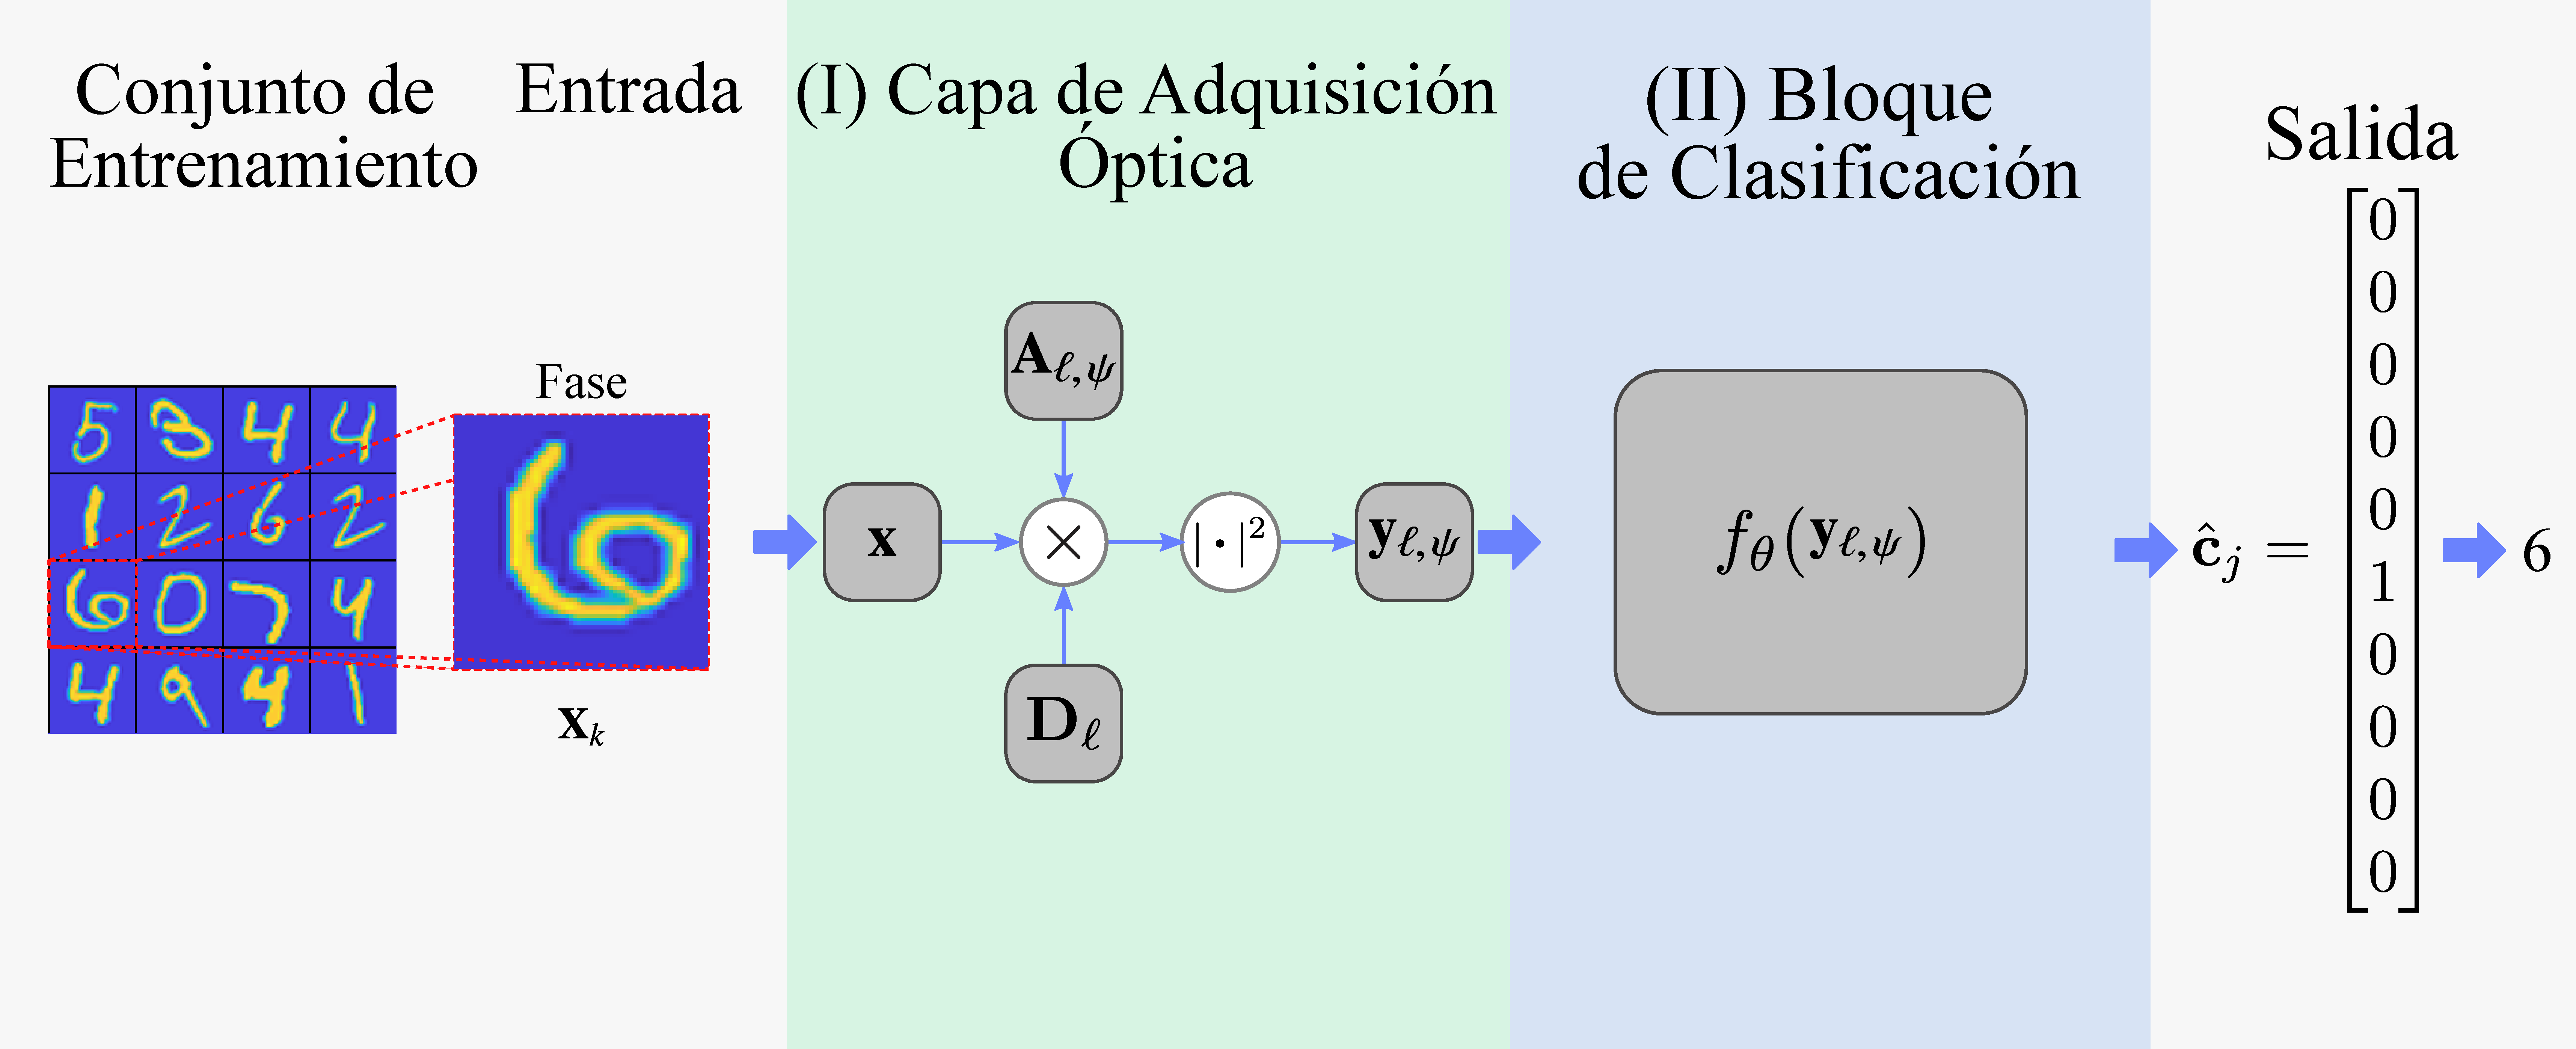
\includegraphics[width=\linewidth]{images/metodología/esquema_entrenamiento_tradicional.pdf}
      \captionof{figure}{Esquema de clasificación usado en el estado del arte.}
        \label{fig:esquema_entrenamiento_tradicional}
    \end{minipage}
    
    En el esquema tradicional no se realiza una modulación del campo óptico, por lo tanto para la comparación con el estado del arte la codificación corresponde a $\mathbf{D}_\ell = 1$.
    
    Adicionalmente se realizó la comparación haciendo uso del operador inverso de la propagación del campo óptico $\mathcal{P}_{\ell, \psi}:\mathbb{C}^n\rightarrow \mathbb{C}^n$ para estimar $\hat{\mathbf{x}}$ \myfootcite{katkovnik2017computational},
    
    \begin{equation}
        \hat{\mathbf{x}}= \frac{1}{L}\sum_{\ell=1}^{ L} \mathcal{P}_{\ell, \psi}(\mathbf{y}_{\ell, \psi}).
        \label{eq:back_propagation}
    \end{equation}
\end{itemize}

\subsection{Configuración experimental}

En esta sección, se presentan los parámetros de simulación utilizados para el modelo de propagación, el bloque de inicialización y la red neuronal de clasificación. La Tabla \ref{tab:parameters} presenta los parámetros ópticos fijados para calcular la matriz $\mathbf{A}_{\ell,\psi}$ \eqref{eq:phase_retrieval_problem} definido en cada campo de difracción. Estos parámetros permiten simular la adquisición de las medidas cuadráticas codificadas a lo largo de cada campo de difracción usando la capa de adquisición óptica. En el bloque de inicialización, el filtro $\mathbf{G} \in \mathbb{C}^{g\times g}$ entrenable fue fijado a un tamaño de kernel $g=5$ y un número de iteraciones $T=10$. Finalmente, el bloque de clasificación fue entrenado usando una tasa de aprendizaje de $1\times 10^{-3}$ con el algoritmo Adam, que requiere $\mathcal{E}=100$ épocas para entrenar sobe los conjuntos de datos MNIST y Fashion-MNIST. Todos los experimentos realizados en este trabajo fueron implementados en \textit{Python 3.9} usando la herramienta \textit{Tensorflow 2.4.1}  \myfootcite{tensorflow2015-whitepaper} para implementar redes neuronales, Los experimentos se ejecutaron sobre un computador con GPU Nvidia 3090 RTX con 64 Gb de memoria RAM y un CPU Intel(R) Xeon(R) W-3223 CPU @ 3.50GHz. El código usado para los experimentos de este trabajo puede ser encontrado de manera pública en el siguiente repositorio 

\begin{table}[!h]
\centering\scalebox{0.9}{
\begin{tabular}{|l|r|r|c|}
\hline
\multicolumn{1}{|c|}{\textbf{Parámetros ópticos}} & \multicolumn{1}{c|}{\textbf{Campo cercano}} & \multicolumn{1}{c|}{\textbf{Campo medio}} & \textbf{Campo lejano} \\ \hline
Longitud de onda ($\lambda$) [nm]                    & 635                           & 635                            & -         \\ \hline
Distancia de propagación ($z$) [cm]         &    2.5                       & 7                              & -         \\ \hline
\end{tabular}}

\caption{ Parámetros de propagación usados para simular el modelo de propagación de la ecuación \eqref{eq:phase_retrieval_problem} para cada campo de difracción.}\label{tab:parameters}
\end{table}


\subsection{Resultados de la inicialización}


la Figura \ref{fig:results_initializations} muestra el desempeño en la métrica de RE del método de estimación inicial propuesto  comparando con los algoritmos FSI, OPI y WMCI variando el número de iteraciones $T$ para los conjuntos de datos MNIST y Fashion-MNIST en los tres campos de difracción, donde se resalta el método propuesto debido a que en todos los casos logra superar los métodos tradicionales obteniendo una estimación inicial en un número menor de iteraciones.

\begin{figure}[h!]
\centering
         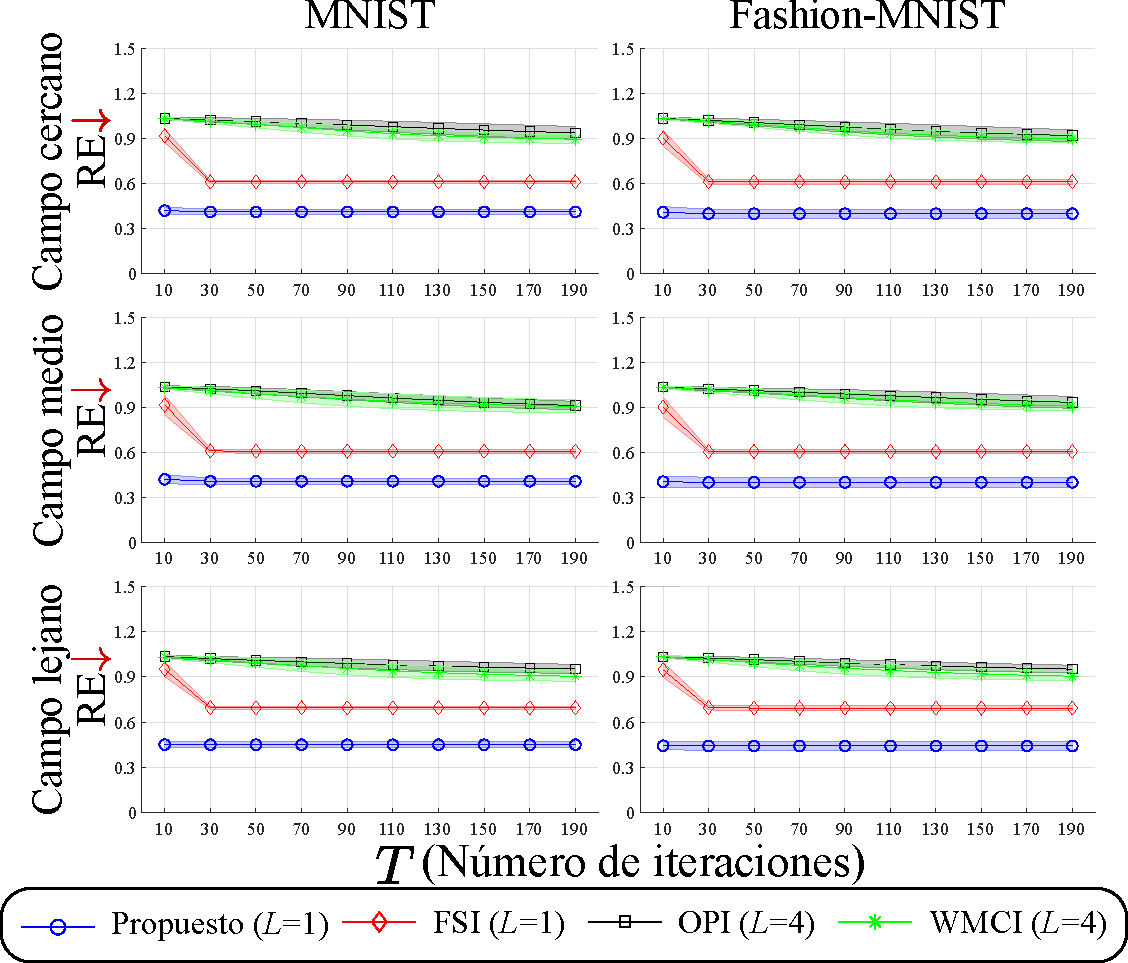
\includegraphics[width=0.8\linewidth]{images/resultados/results_initializations.pdf}
        \caption{Resumen del desempeño de la inicialización propuesta comparando con los métodos FSI, OPI, WMCI sobre la métrica de RE, variando el número de iteraciones del algoritmo para estimar imágenes de los conjuntos MNIST y Fashion-MNIST en los campos de difracción cercano, medio y lejano.}
        \label{fig:results_initializations}
\end{figure}



la Figura \ref{fig:noisy_scenario} muestra la evaluación de la robustés del método frente al ruido, adicionando ruido aditivo gausiano con $SNR = 10, 15$ y $30$. Donde se evidencia que el método propuesto muestra una mayor estabilidad al ruido comparando con los método del estado del arte.

\begin{figure}[h!]
         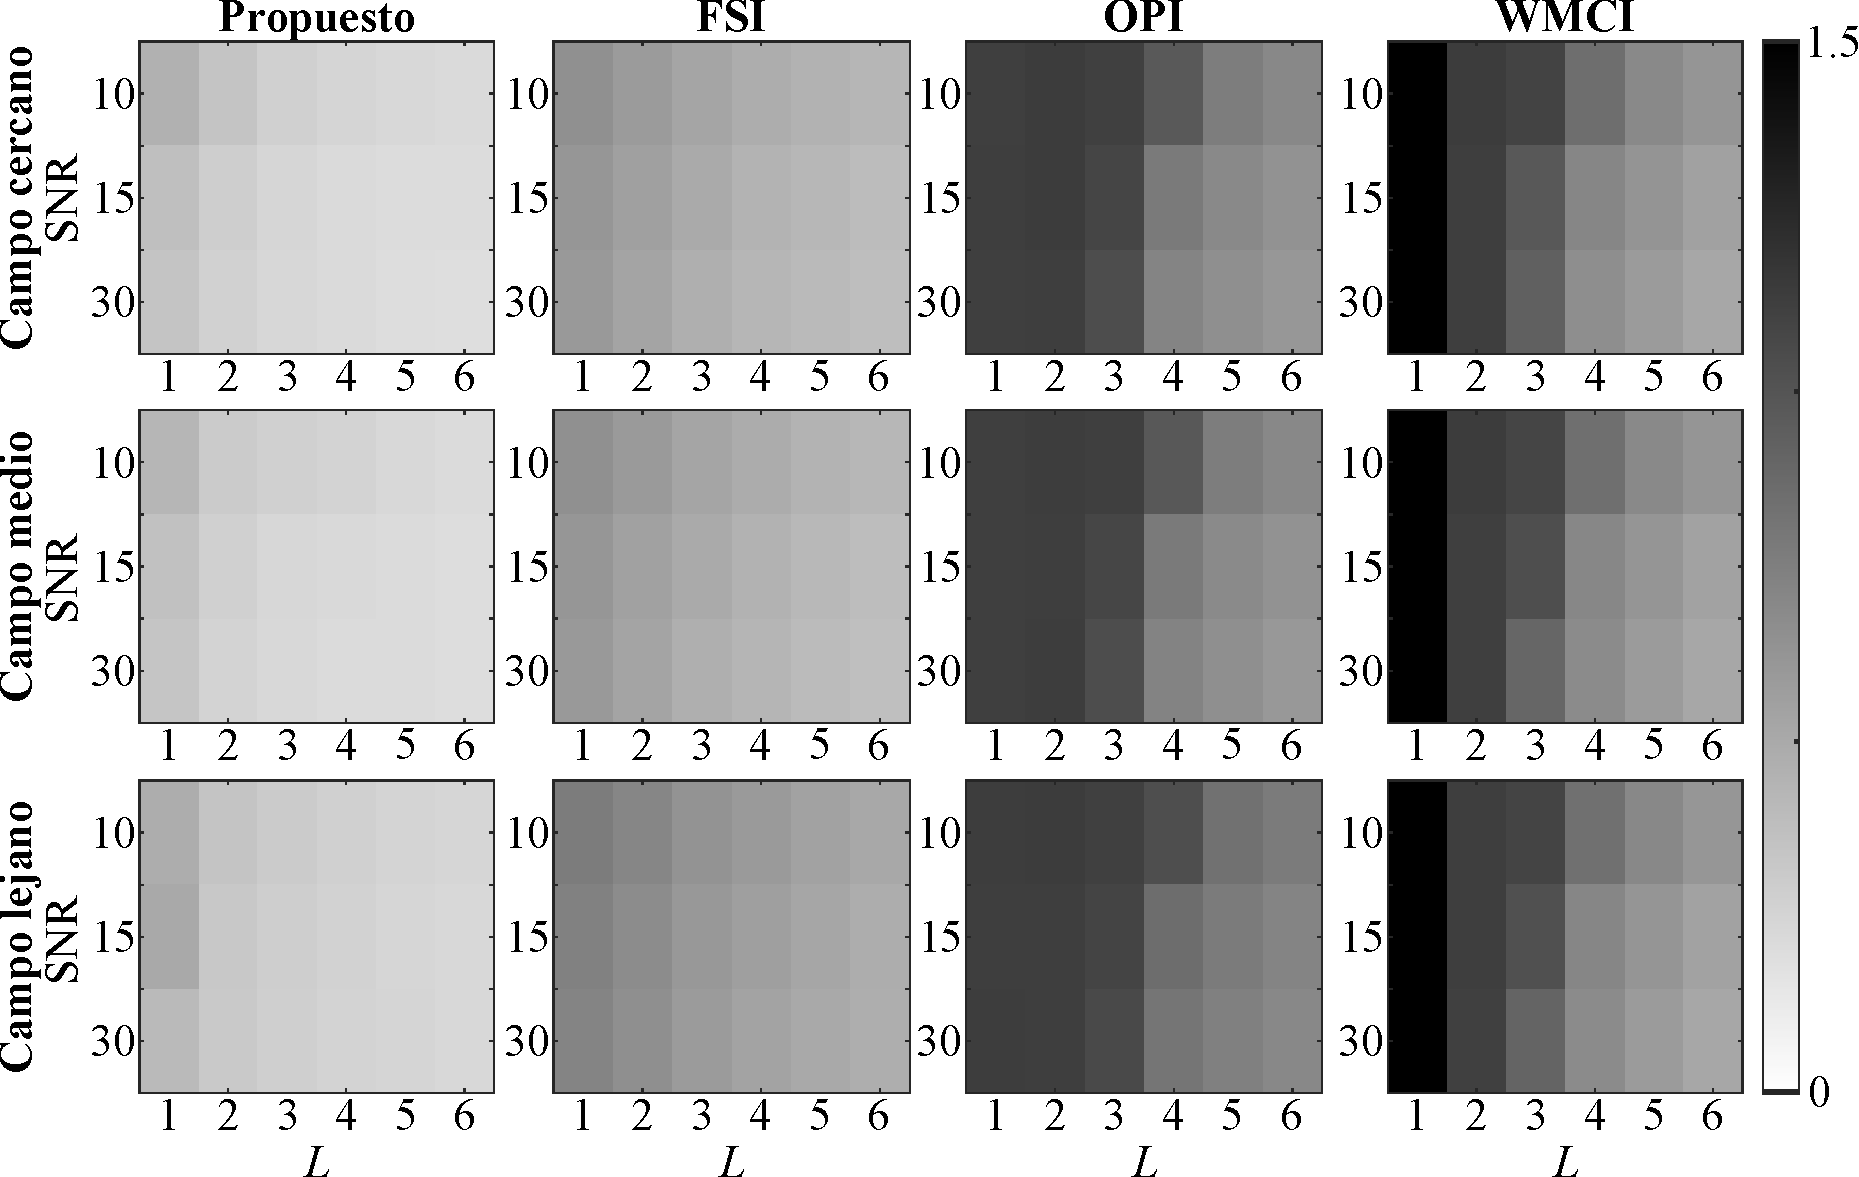
\includegraphics[width=1\linewidth]{images/resultados/Noisy_Initializations.pdf}
        \caption{Resumen del desempeño de la inicialización comparando con diferentes estrategias del estado del arte. Se varió el número de medidas $T$ para realizar la estimación y diferentes niveles de ruido afectando las medidas descritos por el SNR.}
        \label{fig:noisy_scenario}
\end{figure}

Por último, La Figura \ref{fig:resultados_inicialización_sin_ruido} muestra los resultados visuales de la estimación del campo inicial para el conjunto de datos MNIST y Fashion-MNIST. Para comparar el método propuesto se implementaron los algoritmos FSI con $L = 1, T = 10$, FSI usando $L = 1, T=200$, OPI $L = 4, T=200$ y WMCI $L = 4, T=200$. Vale la pena resaltar que el método propuesto logra aproximar el campo óptico en los tres campos de difracción simulados a un bajo número de iteraciones haciendo uso de solo $L=1$ número de medidas y $T=10$ número de iteraciones.

\begin{figure}[!h]
    \centering
    \includegraphics[width=\linewidth]{images/resultados/resultados_inicialización_sin_ruido.pdf}
    \caption{Resultados visuales de la estimación del campo óptico inicial comparando el método propuesto contra el algoritmo FSI con $L = 1, T = 10$, FSI usando $L = 1, T=200$, OPI $L = 4, T=200$ y WMCI $L = 4, T=200$.}
    \label{fig:resultados_inicialización_sin_ruido}
\end{figure}

\subsection{Resultados de la clasificación de objetos}

Los resultados de los experimentos de clasificación se resumen a continuación. Las Figuras \ref{fig:results_acc}, \ref{fig:results_pre},  \ref{fig:results_rec}, \ref{fig:results_f1} muestran los resultados del desempeño de la clasificación de medidas cuadráticas codificadas sobre las métricas de exactitud en la Figura \ref{fig:results_acc}, presición en la Figura \ref{fig:results_pre}, exhaustividad  en la Figura \ref{fig:results_rec} y F1 en la Figura \ref{fig:results_f1}. La clasificación se realizó sobre medidas simuladas en los campos de difracción cercano, medio y lejano. Adicionalmente comparando el método propuesto con la manera tradicional y utilizando un operador inverso sobre las medidas como alternativa a la estimación inicial. Como método de clasificación se usaron las arquitecturas de clasificación MobilNetV2, InceptionV3 y Xception sobre los conjuntos de datos Fashion-MNIST y MNIST.


\begin{figure*}[!h]
    \centering
    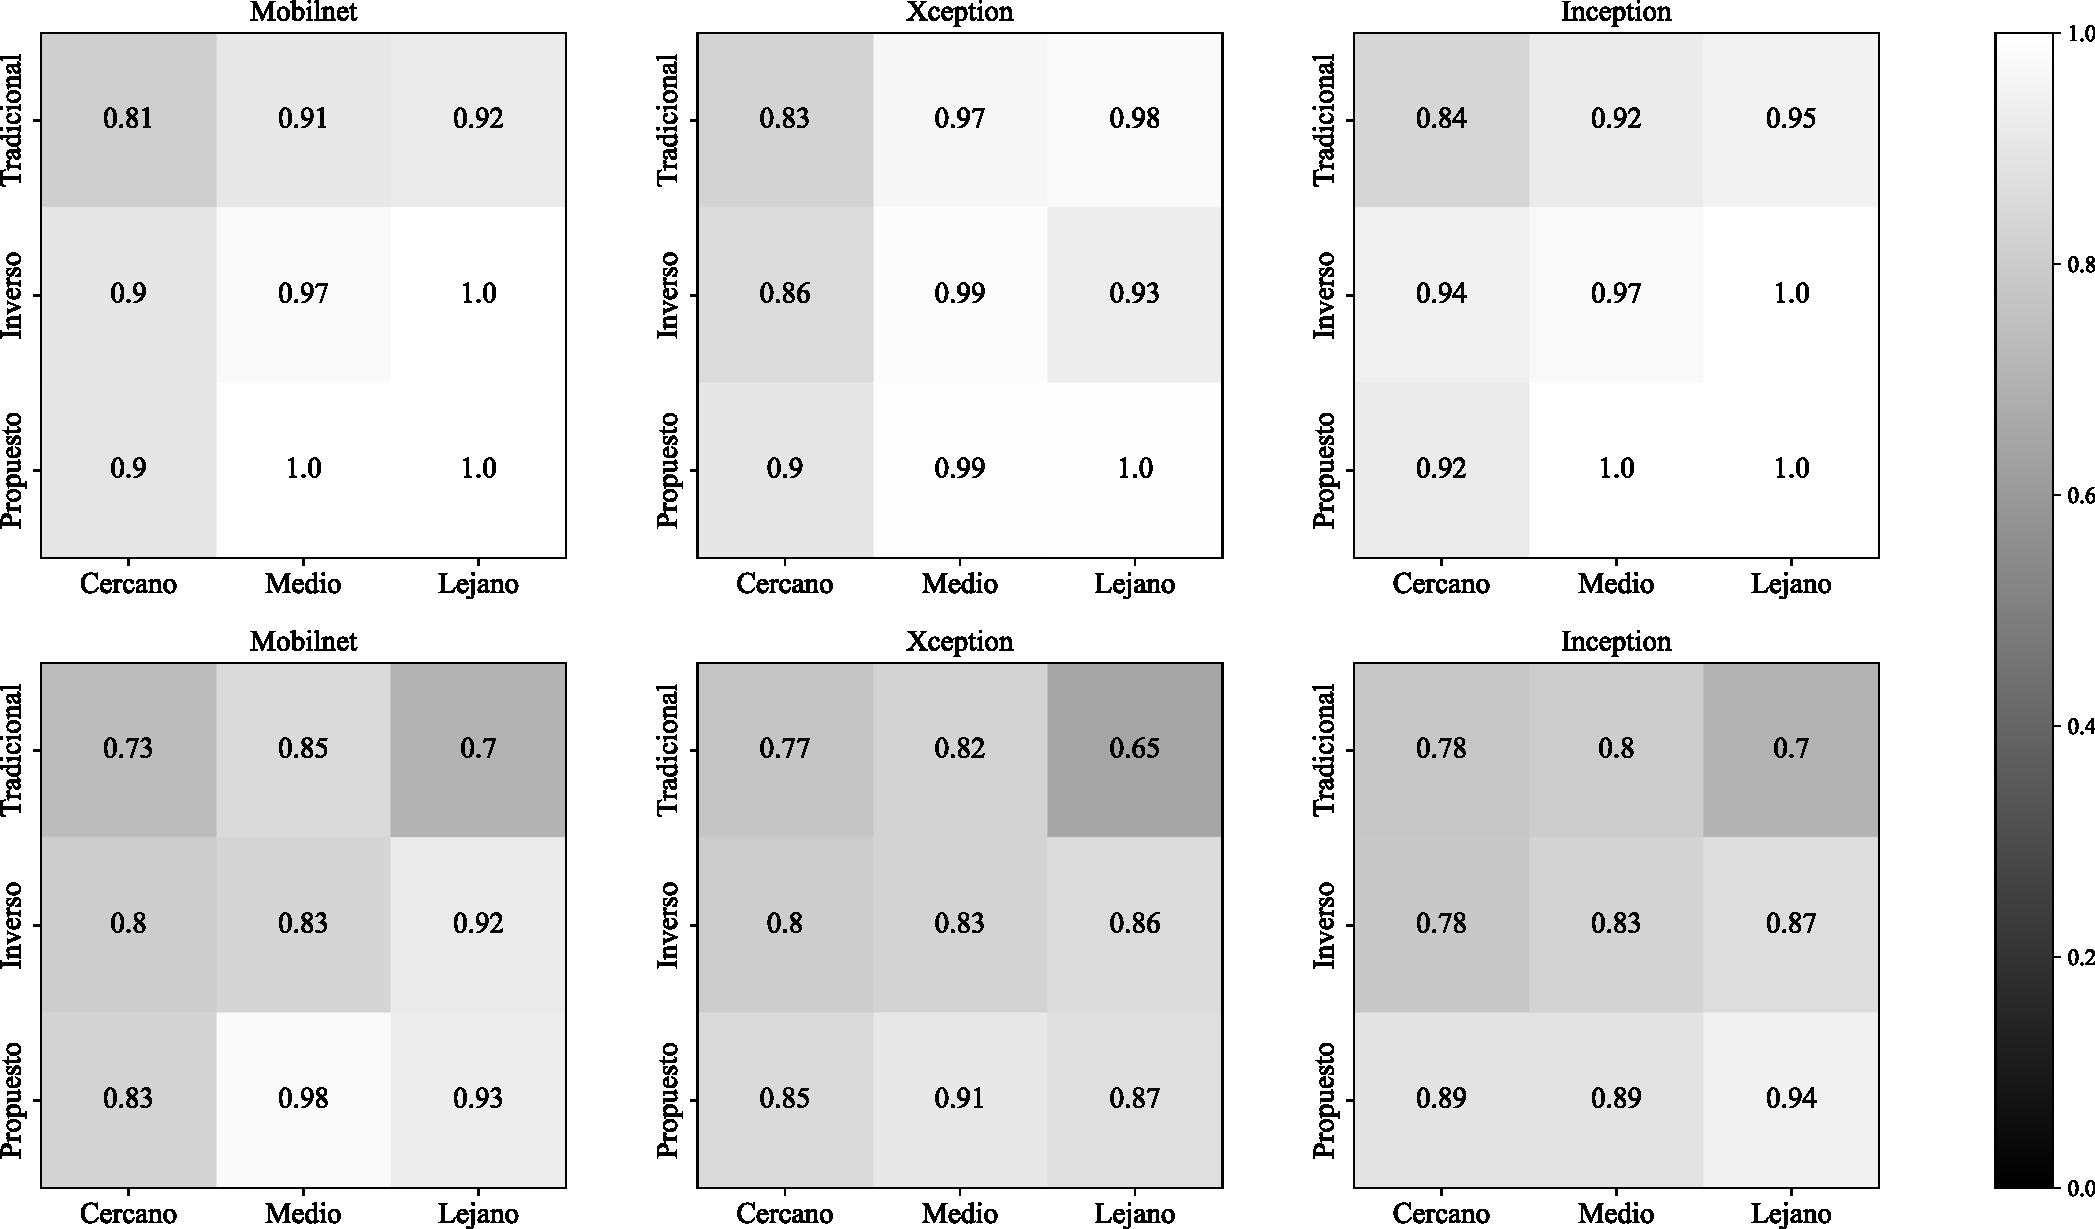
\includegraphics[width=\linewidth]{images/resultados/test_result_Exactitud.pdf}
    \caption{Resultados en la métrica de exactitud para evaluar la clasificación de medidas cuadráticas codificadas simuladas sobre el campo cercano, medio y lejano. Se muestra la comparación de la clasificación tradicional, el uso del propagador inverso y el método propuesto usando las arquitecturas de MobilNetV2, InceptionV3 y Xception sobre la división de prueba de los conjuntos de datos MNIST y Fashion-MNIST.}
    \label{fig:results_acc}
\end{figure*}

\begin{figure*}[!h]
    \centering
    \includegraphics[width=\linewidth]{images/resultados/test_result_Presición.pdf}
    \caption{Resultados en la métrica de presición para evaluar la clasificación de medidas cuadráticas codificadas simuladas sobre el campo cercano, medio y lejano. Se muestra la comparación de la clasificación tradicional, el uso del propagador inverso y el método propuesto usando las arquitecturas de MobilNetV2, InceptionV3 y Xception sobre la división de prueba de los conjuntos de datos MNIST y Fashion-MNIST.}
    \label{fig:results_pre}
\end{figure*}



\begin{figure*}[!h]
    \centering
    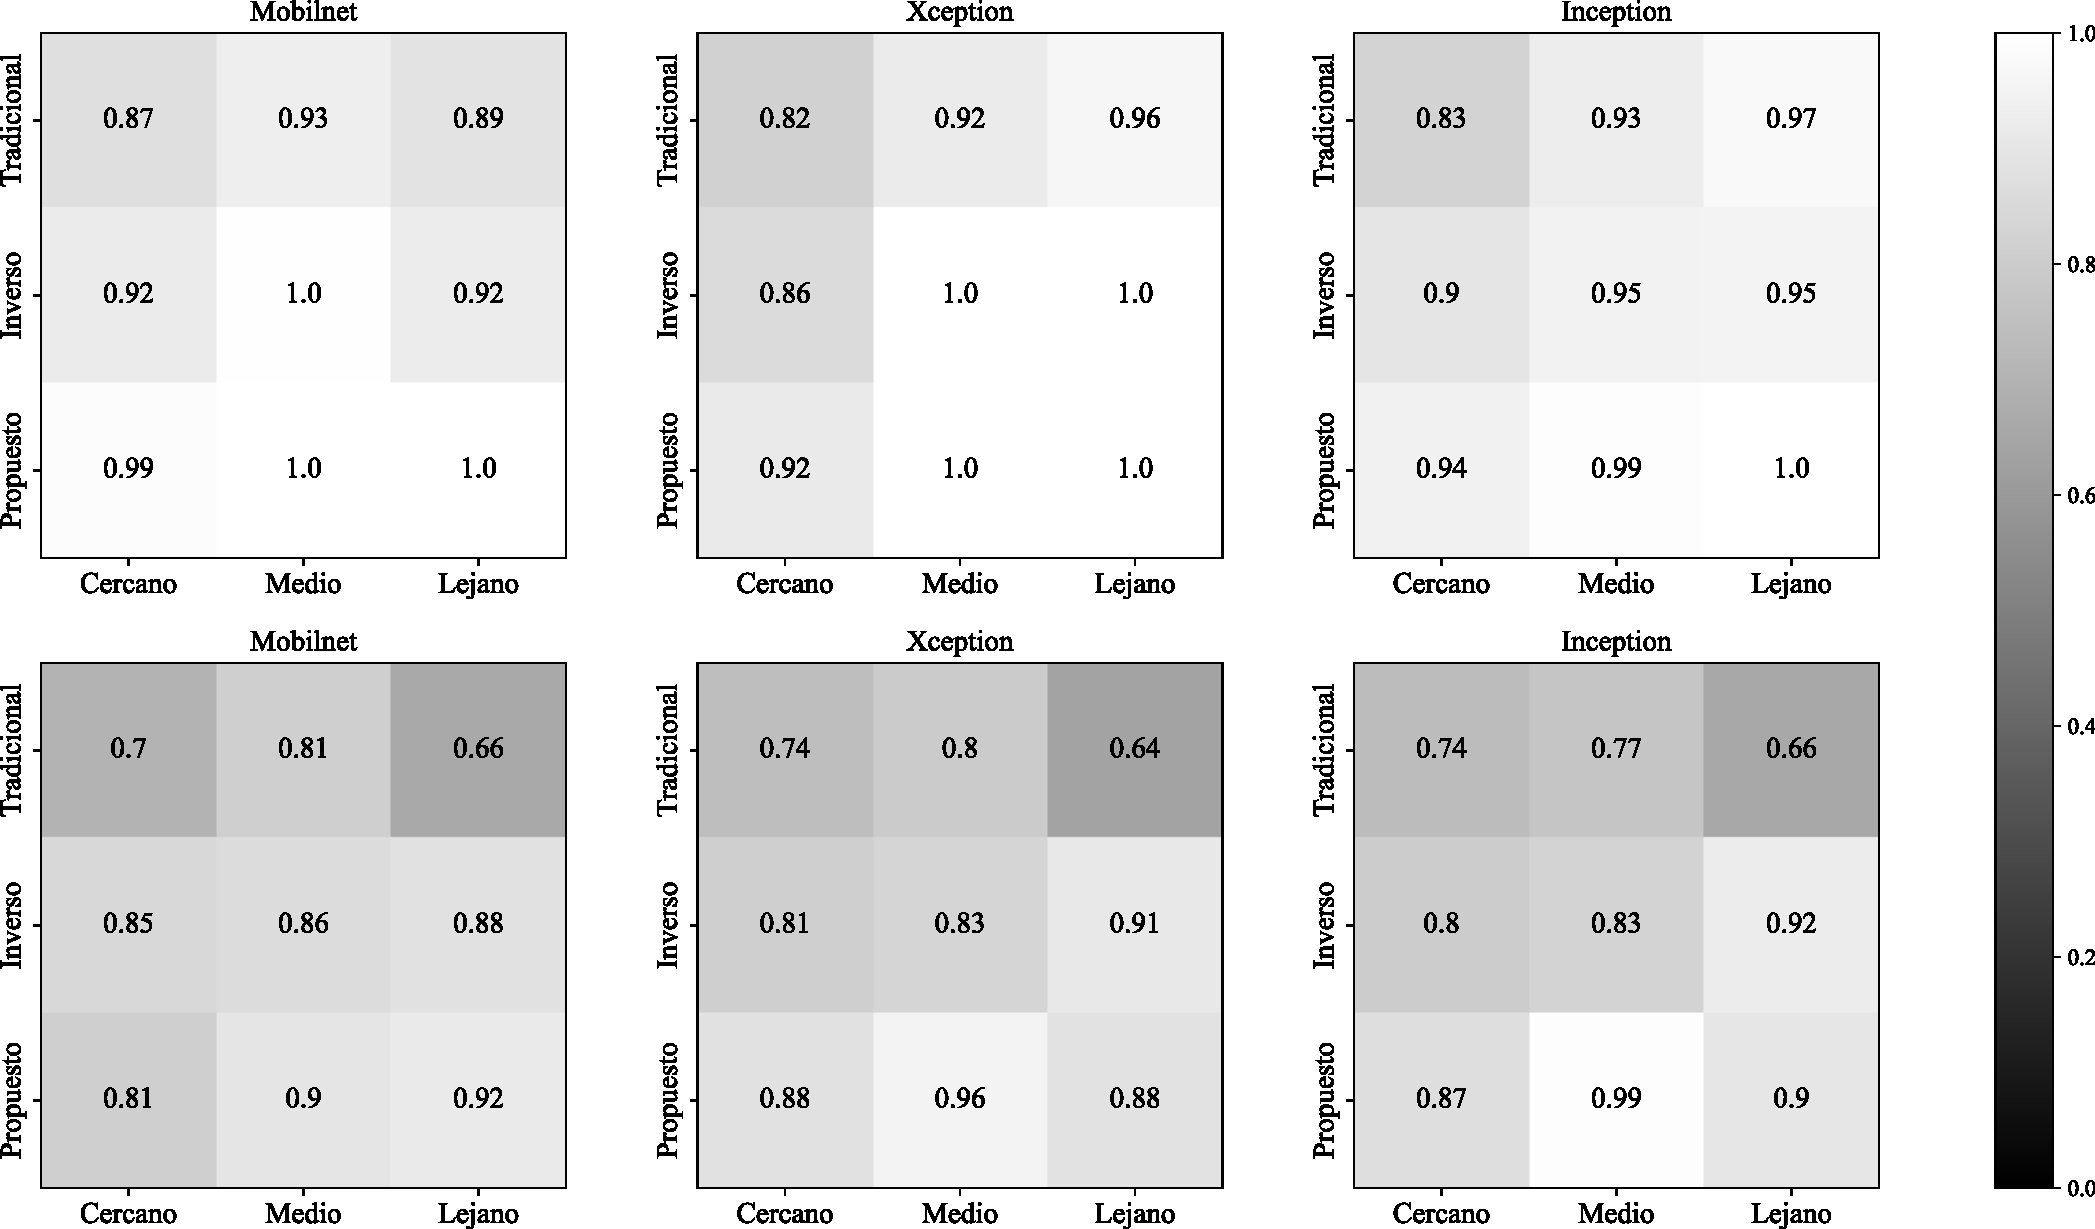
\includegraphics[width=\linewidth]{images/resultados/test_result_Exhaustividad.pdf}
    \caption{Resultados en la métrica de exhaustividad para evaluar la clasificación de medidas cuadráticas codificadas simuladas sobre el campo cercano, medio y lejano. Se muestra la comparación de la clasificación tradicional, el uso del propagador inverso y el método propuesto usando las arquitecturas de MobilNetV2, InceptionV3 y Xception sobre la división de prueba de los conjuntos de datos MNIST y Fashion-MNIST.}
    \label{fig:results_rec}
\end{figure*}

\begin{figure*}[!h]
    \centering
    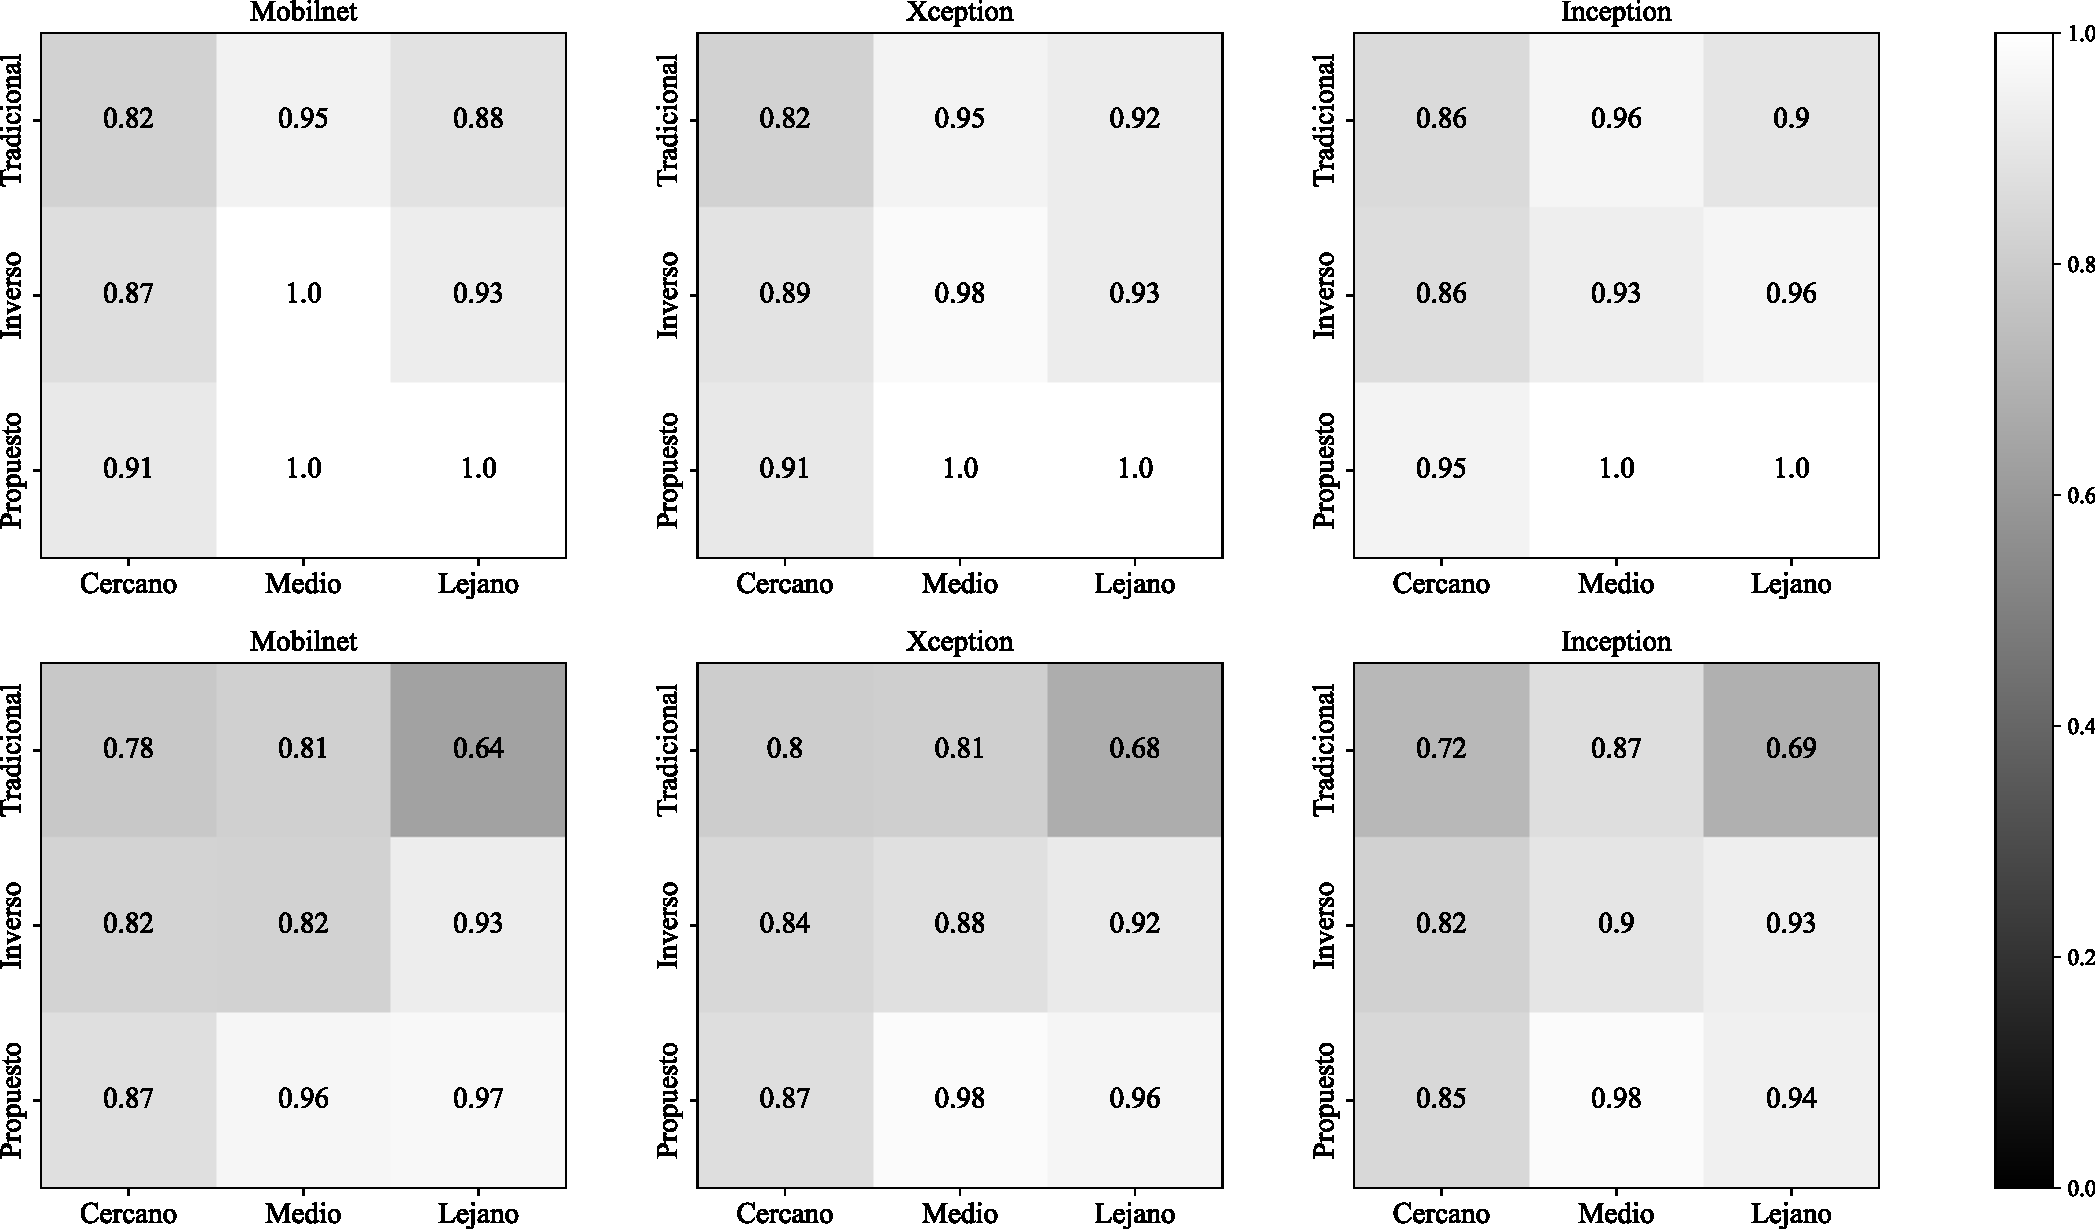
\includegraphics[width=\linewidth]{images/resultados/test_result_F1.pdf}
    \caption{Resultados en la métrica de F1 para evaluar la clasificación de medidas cuadráticas codificadas simuladas sobre el campo cercano, medio y lejano. Se muestra la comparación de la clasificación tradicional, el uso del propagador inverso y el método propuesto usando las arquitecturas de MobilNetV2, InceptionV3 y Xception sobre la división de prueba de los conjuntos de datos MNIST y Fashion-MNIST.}
    \label{fig:results_f1}
\end{figure*}